\section{Multi-objective analysis: cost, speed and CO$_2$}\label{sec:pareto}

The late penalty $\lambda$ is not a cost that appears on an invoice.
It is a \emph{policy choice} about how much the business is willing to pay for the next-day promise.
Rather than fixing it, we trace the trade-off for a representative regular day (5 March 2026).
All plans are evaluated out of sample on 2000 true scenarios.
Each plan is operated with the price of speed it was planned with, so the recourse assignment is consistent with the plan.

\paragraph{Methods.}
\begin{enumerate}
  \item \textbf{Weighted sum}: solve the SAA ($N=100$, Benders) for 13 values of $\lambda\in[0,20]$ \EUR{}/late unit.
  \item \textbf{Augmented $\varepsilon$-constraint}, on a 10-scenario SAA solved exactly as an extensive form. Minimise cost subject to $\sum_s p_s(\text{late}_s + \text{unshipped}_s)\le\varepsilon\sum_s p_s D_s$, for 16 equally spaced values of $\varepsilon$ between the two extremes of the weighted sum. A tiny tie-breaking penalty ($10^{-3}$ \EUR{}/unit) on lateness removes weakly efficient solutions, which is what AUGMECON's slack term achieves \citep{mavrotas2009,mavrotas2013}.

  Because the $\varepsilon$-constraint couples all scenarios, a plan obtained this way does not by itself say how to operate on a given day. We therefore re-solve the LP with the integer first stage fixed and read the Lagrange multiplier $\lambda^\star_\varepsilon$ of the $\varepsilon$-row. By LP duality, a recourse that prices lateness at $\lambda^\star_\varepsilon$ reproduces the planned service level; we verified this numerically to five digits. $\lambda^\star_\varepsilon$ is also the \emph{marginal price of the last point of speed} at that point of the frontier.
  \item \textbf{Carbon price}: add $\kappa$ \EUR{}/t CO$_2$ to the line-haul cost per truck-km, for $\kappa$ up to \EUR{3200}/t.
\end{enumerate}

\begin{figure}[t]
  \centering
  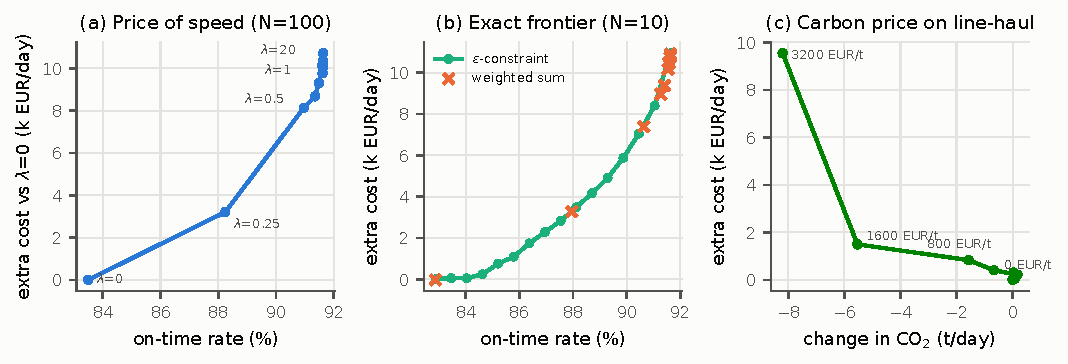
\includegraphics[width=\linewidth]{pareto}
  \caption{(a) Out-of-sample cost--speed frontier from the weighted-sum sweep. (b) Exact in-sample frontier from the $\varepsilon$-constraint method (16 points) and the weighted-sum solutions on the same 10-scenario SAA. The weighted sum clusters at the ends; the $\varepsilon$-constraint covers the frontier evenly. (c) Cost--CO$_2$ trade-off under a carbon price on line-haul trucks.}
  \label{fig:pareto}
\end{figure}

\needspace{5\baselineskip}
\paragraph{Findings.}
\begin{enumerate}
  \item \textbf{Speed is cheap, until it is impossible.} Moving from the cheapest plan ($\lambda=0$, 83.5\% on time) to $\lambda=0.5$ (91.0\%) costs only \EUR{8.1}k per day (0.36\%). The frontier then turns vertical at 91.6\%. The last 8.4\% of units cannot be delivered next day at any price on this day: their zones are reachable on time only from FCs that lack the inventory or capacity (\cref{fig:planmap}). This is a \emph{network design} limit, not an operational one; \cref{sec:network} prices the investment that moves it.
  \item \textbf{Speed is bought in the assignment layer.} Across the whole frontier the plan keeps 516--523 trucks and 251--253 crews. Faster plans route differently through the same capacity rather than buying more. This is useful for leadership communication: the promise level is mostly an \emph{operational} decision that can be changed daily, without re-sizing the network.
  \item \textbf{Marginal prices along the frontier.} The multipliers $\lambda^\star_\varepsilon$ grow from \EUR{0.003} to \EUR{0.42} per late unit up to 90\% on time, and reach \EUR{1.98} for the last attainable point. The default $\lambda=\EUR{1}$ therefore sits at the knee of the frontier.
  \item \textbf{Weighted sum vs.\ $\varepsilon$-constraint.} With integer trucks the frontier could in principle be non-convex, with unsupported points that no weighted sum can reach. We tested this against the lower convex hull of all 29 exact solutions. Eight $\varepsilon$-points lie above the hull, but by at most \EUR{125} on \EUR{2.27}M, which is below the MIP tolerance. The frontier is therefore convex for practical purposes. The value of the $\varepsilon$-method here is \emph{coverage}: seven of the 13 weighted-sum solutions collapse onto practically the same point at $\lambda\ge 2$, whereas the $\varepsilon$-constraint delivers evenly spaced options, each with its marginal price.
  \item \textbf{Line-haul carbon is expensive to abate.} A carbon price below \EUR{400}/t changes nothing: trucks are already well consolidated, and the lanes are fixed by geography. At \EUR{1600}--\EUR{3200}/t the plan sheds 10--23 trucks and cuts 5.5--8.2\,t of CO$_2$ per day (6--9\% of line-haul emissions of about 92\,t; last mile adds 77\,t that the plan cannot influence). It does so by consolidating volume onto fewer, fuller trucks and shifting the overflow to spot capacity. This costs \EUR{1.5}--\EUR{9.5}k per day, an implied abatement cost of \EUR{270}--\EUR{1160}/t before counting the 1.3--2.2 points of on-time delivery that are lost. Speed itself has a carbon cost: the next-day plan ($\lambda=1$) emits 7.3\,t (4.5\% of total, 8\% of line-haul) more CO$_2$ than the cheapest plan ($\lambda=0$), because on-time lanes are often longer ones.
\end{enumerate}
